%%
% La siguiente plantilla esta basada en el siguiente enlace:
% http://academic.reed.edu/physics/courses/Physics332.s08/reports.html
% La plantilla original puede descargarse de ese sitio
% Se dejo parte del texto original en inglés para ilustar el uso de la plantilla
% Se hicieron algunas modificaciones para ajustar el idioma y otros detalles para 
% completar un reporte técnico breve pero muy puntual
% Modificación Inicial: Marco Aurelio Nuno Maganda - 11/SEP/2014
% 
% Enlace a la documentación del tipo de documento base (revtex4)
% http://mirror.hmc.edu/ctan/macros/latex/contrib/revtex/doc/latex/revtex/source/revtex4-1.pdf
%
% En algunas distribuciones es necesario instalar el paquete texlive-publishers
%
%\documentclass[letterpaper,aps,twocolumn,pre,nofootinbib]{revtex4}
%\documentclass[twocolumn]{article}
\documentclass[conference]{IEEEtran}

\usepackage[spanish]{babel}
\usepackage{amsmath,amssymb,amsfonts,amsthm}
\usepackage{graphicx}
%\usepackage{bbm}
\usepackage[utf8]{inputenc} % Caracteres en Español (Acentos, ñs)
\usepackage{url} % ACENTOS
\usepackage{hyperref} % Referencias
\usepackage{subfig}
\usepackage{lipsum}
\usepackage{balance}
\usepackage{float} 


%%%%%%%%%%%%%%%%%%%%%%%%%%%%%%%%%%%%%%%%%%%%%
% PARCHE PARA ELIMINAR LA FECHA DEL DOCUMENTO
% 
\usepackage{etoolbox}
\makeatletter
% \frontmatter@RRAP@format is responsible for the parentheses
\patchcmd{\frontmatter@RRAP@format}{(}{}{}{}
\patchcmd{\frontmatter@RRAP@format}{)}{}{}{}
%\renewcommand\Dated@name{}
\makeatother	
% FIN DEL PARCHE
% 
%%%%%%%%%%%%%%%%%%%%%%%%%%%%%%%%%%%%%%%%%%%%%

%%%%%%%%%%%%%%%%%%%%%%%%%%%%%%%%%%%%%%%%%%%%%
% PARCHE PARA PERMIRIR UTILIZAR BIBLATEX EN ESTA PANTLLA
%\PassOptionsToPackage{square,numbers}{natbib}
%\RequirePackage{natbib}  
%%%%%%%%%%%%%%%%%%%%%%%%%%%%%%%%%%%%%%%%%%%%%

\usepackage[backend=bibtex,sorting=none]{biblatex}
% Estas lineas permiten romper los hipervinculos muy largos !!!!
\setcounter{biburllcpenalty}{7000}
\setcounter{biburlucpenalty}{8000}
\addbibresource{references.bib}

% Actualiza en automático la fecha de las citas de internet a la fecha de la compilación del documento
\usepackage{datetime}
\newdateformat{specialdate}{\twodigit{\THEDAY}-\twodigit{\THEMONTH}-\THEYEAR}
\date{\specialdate\today}

% la sentencia \burl en las citas... 
\usepackage[hyphenbreaks]{breakurl}

\renewcommand\spanishtablename{Tabla}
\renewcommand\spanishfigurename{Figura}

%\usepackage{datetime}
%\newdateformat{specialdate}{\twodigit{\THEDAY}-\twodigit{\THEMONTH}-\THEYEAR}
%\newdateformat{specialdate}{\twodigit{\THEDAY}-\THEYEAR}
%\date{\specialdate\today}


\begin{document}
%%%%%%%%%%%%%%%%%%%%%%%%%%%%%%%%%%%%%%%%%%%%%
% Definitions
%
%
% Define your special symbols here
%
%%%%%%%%%%%%%%%%%%%%%%%%%%%%%%%%%%%%%%%%%%%%%

% use to set width of figures
\newcommand{\breite}{0.9} %  for twocolumn
\newcommand{\RelacionFiguradoscolumnas}{0.9}
\newcommand{\RelacionFiguradoscolumnasPuntoCinco}{0.45}


%%%%%%%%%%%%%%%%%%%%%%%%%%%%%%%%%%%%%%%%%%%%%
% End Definitions
%%%%%%%%%%%%%%%%%%%%%%%%%%%%%%%%%%%%%%%%%%%%%


%Title of paper
\title{Reporte de Laboratorio III \\  Skeletal Animation
}

% Trabajo Individual
\author{
\IEEEauthorblockN{Bocanegra González Carlos Antonio\IEEEauthorrefmark{1}, Coyoy López Mario\IEEEauthorrefmark{1},  \\
Nava López Heriberto Geovanny\IEEEauthorrefmark{1}, Rivera Zamarrón Nuria Yaretzi\IEEEauthorrefmark{1}}

% En caso de trabajos en equipo, poner a todos los autores en estricto ORDEN ALFABETICO
%\author{\IEEEauthorblockN{Michael Shell\IEEEauthorrefmark{1},
%Homer Simpson\IEEEauthorrefmark{1},
%James Kirk\IEEEauthorrefmark{1}, 
%Montgomery Scott\IEEEauthorrefmark{1} and
%Eldon Tyrell\IEEEauthorrefmark{1}}
\IEEEauthorblockA{\IEEEauthorrefmark{1}Ingeniería en Tecnologías de la Información\\
Universidad Politécnica de Victoria}
}


%\date{}

\maketitle

\begin{abstract}  
\textbf{El proyecto consistió en desarrollar una aplicación móvil para Android que permite visualizar y animar modelos 3D en tiempo real utilizando el motor Filament y OpenGL. La aplicación incluye una interfaz de usuario intuitiva con controles táctiles para rotar, hacer zoom y trasladar la cámara, así como un control deslizante para manipular el tiempo de las animaciones. Los modelos 3D, como personajes y dinosaurios, fueron optimizados para dispositivos móviles mediante la reducción de polígonos y la compresión de texturas. Además, se implementaron animaciones esqueléticas, asegurando movimientos fluidos y realistas. La calidad gráfica se mejoró con shaders avanzados que añaden iluminación y sombras realistas. \cite{android-os}
}
\end{abstract}


%\maketitle must follow title, authors, abstract, \pacs, and \keywords

\section{Introducción}  
Este proyecto tiene como objetivo crear una aplicación móvil en Android \cite{android-dev} desarrolada usando el lenguaje de programación Koltin \cite{kotlin} que permita la visualización y animación de modelos 3D utilizando el motor de renderizado Filament, basado en OpenGL. \cite{opengl} La aplicación implementa animaciones esqueléticas (Skeletal Animation), una técnica utilizada para animar modelos 3D de manera eficiente, manipulando un \textit{esqueleto} de huesos virtuales en lugar de mover vértices directamente. Este enfoque es ideal para personajes complejos, como los modelos 3D descargados de internet, que en su mayoría se presentan en formatos como \textit{.blend} o \textit{.fbx}, los cuales fueron convertidos a \textit{glb/glTF} utilizando la herramienta Blender para asegurar su compatibilidad con la aplicación.
La animación esquelética en la aplicación se ha implementado en combinación con el uso de cámaras, perspectiva y shaders personalizados, lo que permite una visualización realista y dinámica de los modelos 3D en tiempo real. Los modelos seleccionados incluyen personajes como un ratón, un dinosaurio T-Rex y un vampiro, los cuales fueron creados y animados a través de esta técnica. La interfaz de usuario desarrollada integra la visualización interactiva, permitiendo al usuario controlar la animación mediante una barra de tiempo.
Este reporte presenta los detalles del diseño, la implementación y los desafíos que se enfrentaron al trabajar con diferentes tecnologías y formatos de modelos 3D, como .glb y glTF, en un entorno móvil. Además, se discuten las aplicaciones prácticas de este enfoque para el desarrollo de experiencias interactivas y educativas en dispositivos móviles. \cite{androidTutorial}


\section{Desarrollo Experimental}

En este proyecto, el objetivo principal era crear una aplicación móvil para visualizar y animar modelos 3D, utilizando el motor de renderizado Filament, basado en OpenGL \cite{opengles}, en una plataforma Android. Se describen en detalle los diferentes componentes y fases del desarrollo experimental, incluyendo los aspectos técnicos de la implementación y los procesos de trabajo involucrados.

\subsection{1. Selección de la Tecnología y Herramientas}

La elección de las herramientas y tecnologías fue fundamental para lograr el objetivo del proyecto. El motor Filament \cite{filamentGraphics} se eligió debido a su capacidad para ofrecer gráficos de alta calidad en dispositivos móviles, siendo compatible con OpenGL, que es la API gráfica de bajo nivel utilizada en Android para la renderización de gráficos en 3D.

\subsubsection{Filament y OpenGL}

Filament es un motor de renderizado que permite crear imágenes y animaciones 3D de alta calidad, utilizando técnicas avanzadas como la iluminación basada en física (PBR). Es ideal para este tipo de proyectos en Android, ya que proporciona un balance entre la calidad visual y el rendimiento, crucial para dispositivos móviles con limitaciones de hardware.

Por otro lado, OpenGL se usa para la creación de gráficos 3D y se integra con Filament para realizar la renderización eficiente de las escenas en tiempo real. Aunque OpenGL es una API relativamente antigua, su amplia compatibilidad y eficiencia para gráficos en dispositivos móviles lo convierten en una herramienta esencial para este proyecto.

\subsection{2. Modelos 3D y Conversión de Formatos}

Los modelos 3D utilizados en este proyecto fueron descargados de internet en formatos como .fbx, que es ampliamente usado en el desarrollo de videojuegos y animaciones 3D. Sin embargo, estos modelos no son compatibles directamente con Filament, por lo que se tuvo que realizar una conversión del formato .fbx a .glb/glTF, más eficiente y compatible.

\subsubsection{Uso de Blender para la Conversión}

Blender, un software de modelado y animación 3D de código abierto, se utilizó para convertir los modelos de .fbx a .glb. Los pasos incluyeron:

\begin{enumerate}
    \item Importación del archivo .fbx o .blend a Blender.
    \item Revisión de las animaciones esqueléticas y las texturas.
    \item Exportación a formato .glb/glTF, asegurando que las animaciones y texturas se mantuvieran intactas.
\end{enumerate}

\subsection{3. Animación Esquelética (Skeletal Animation)}

La animación esquelética es una técnica que utiliza huesos virtuales para mover un modelo 3D de manera eficiente. Este método es ideal para personajes complejos, ya que permite un control detallado sobre la animación.

\subsubsection{Implementación de la Animación Esquelética}

Filament se usó para cargar los modelos .glb, los cuales contenían las animaciones esqueléticas. La aplicación fue diseñada para reproducir estas animaciones en tiempo real, asegurando un movimiento fluido y natural.

\subsection{4. Implementación de la Interfaz de Usuario}

La aplicación fue desarrollada utilizando Android Studio, y la interfaz de usuario se diseñó para ser sencilla e intuitiva. Incluye:

\begin{itemize}
    \item Visualización del modelo 3D en tiempo real.
    \item Barra de control para manipular la animación.
    \item Gestos táctiles para rotar, hacer zoom y trasladar la cámara.
    \item Botón para reiniciar la posición y el área de interés de la cámara.
\end{itemize}

\subsection{5. Optimización para Móviles}

Para asegurar un rendimiento fluido, se realizaron optimizaciones como:

\begin{itemize}
    \item Reducción de la complejidad de los modelos.
    \item Uso eficiente de texturas comprimidas.
    \item Compresión de animaciones mediante interpolación de cuadros clave.
\end{itemize}

\subsection{6. Visualización y Perspectiva}

La visualización en 3D y la perspectiva fueron claves en este proyecto. Se implementó una cámara virtual con gestos táctiles y shaders para mejorar los efectos visuales, incluyendo sombras y detalles de iluminación.

\subsection{7. Pruebas y Resultados}

Se realizaron pruebas de funcionalidad y rendimiento, logrando:

\begin{itemize}
    \item Rendimiento estable en dispositivos de gama media.
    \item Animaciones reproducidas sin errores.
    \item Interfaz responsiva e intuitiva.
\end{itemize}


%%%%%%%%%%%%%%%%%%%%%%%%%%%%%%%%%%%%%%%%%%%%%%%%%%%%
\section{Resultados}

El desarrollo de la aplicación para la visualización y animación de modelos 3D permitió obtener resultados funcionales y estéticamente satisfactorios en dispositivos móviles con Android \cite{gameDevAndroid}. Se presentan los principales resultados obtenidos, respaldados por capturas de pantalla que ilustran las características implementadas:

\subsection{Interfaz de Usuario Intuitiva}

La interfaz principal, como se muestra en la figura \ref{fig:interfaz_inicial}, fue diseñada para ser limpia y funcional, permitiendo al usuario acceder a las opciones principales sin dificultad. Se incluyó un botón de \textit{Reiniciar cámara} para restablecer la perspectiva del modelo 3D, lo cual resultó útil durante las pruebas de interacción. Además, se implementó un control deslizante que permite manipular el tiempo de animación en los modelos, mejorando la experiencia del usuario.

\begin{figure}[H]
    \centering
    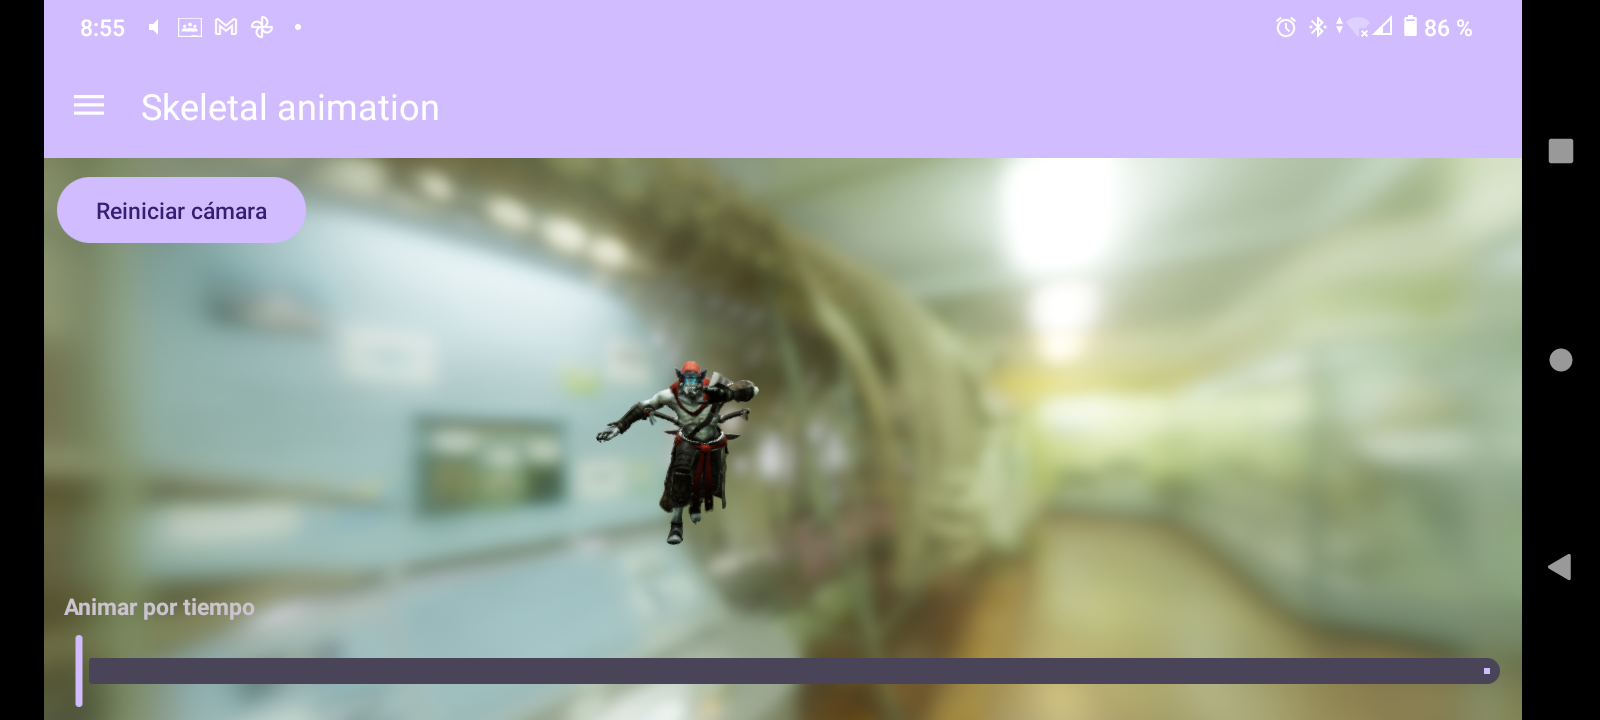
\includegraphics[width=0.45\textwidth]{img/Captura_1.png}
    \caption{Vista inicial de la aplicación mostrando el control deslizante y el botón de reinicio de cámara.}
    \label{fig:interfaz_inicial}
\end{figure}

\subsection{Visualización de Animaciones Esqueléticas}

Los modelos 3D animados, como un personaje humanoide y un dinosaurio, fueron renderizados \cite{pbrOverview} con precisión utilizando Filament y OpenGL. Las animaciones esqueléticas se reprodujeron correctamente, permitiendo movimientos suaves y sin distorsiones. Esto fue probado en diversas secuencias de animación.

\begin{figure}[H]
    \centering
    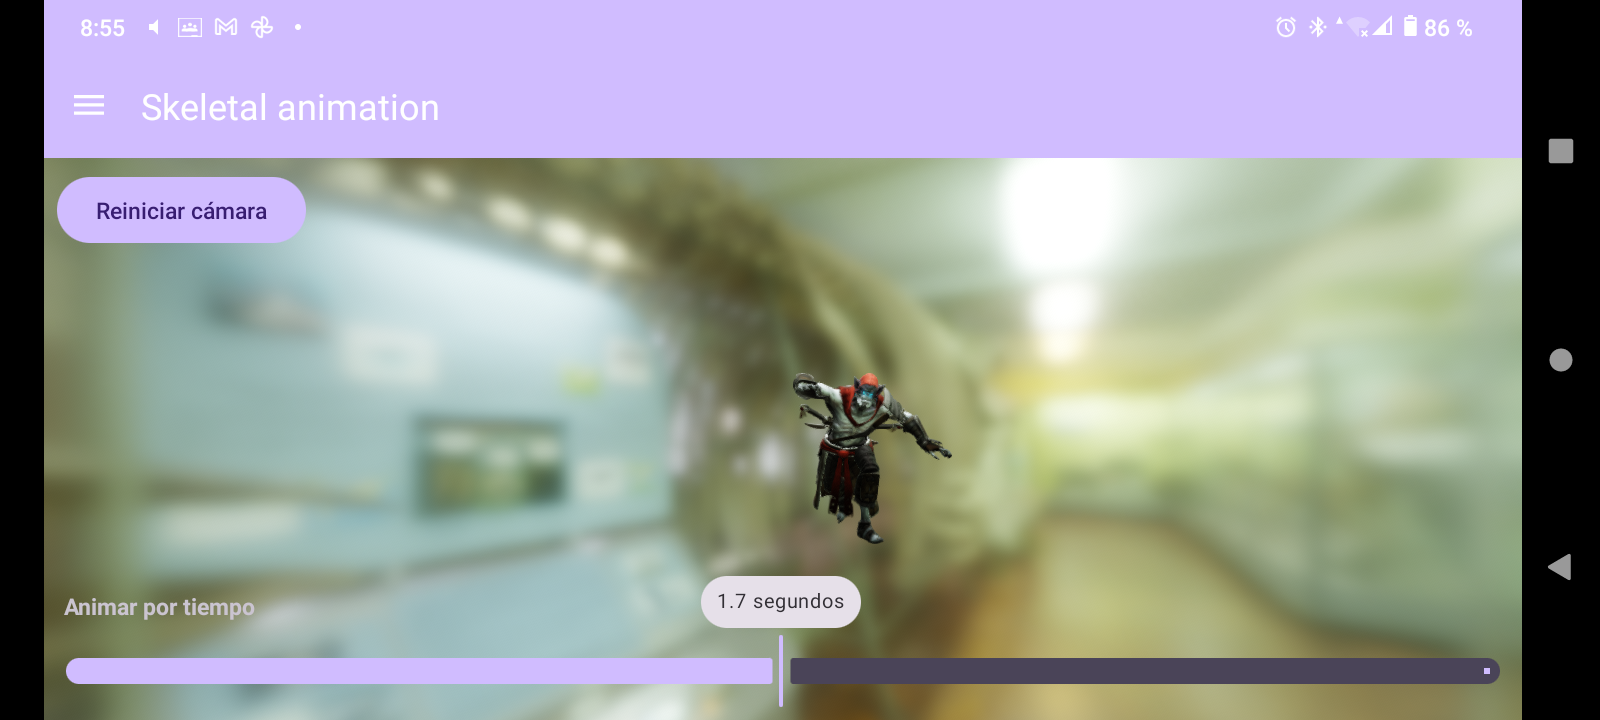
\includegraphics[width=0.45\textwidth]{img/Captura_2.png}
    \caption{Modelo humanoide animado en tiempo real.}
    \label{fig:modelo_humanoide}
\end{figure}

\begin{figure}[H]
    \centering
    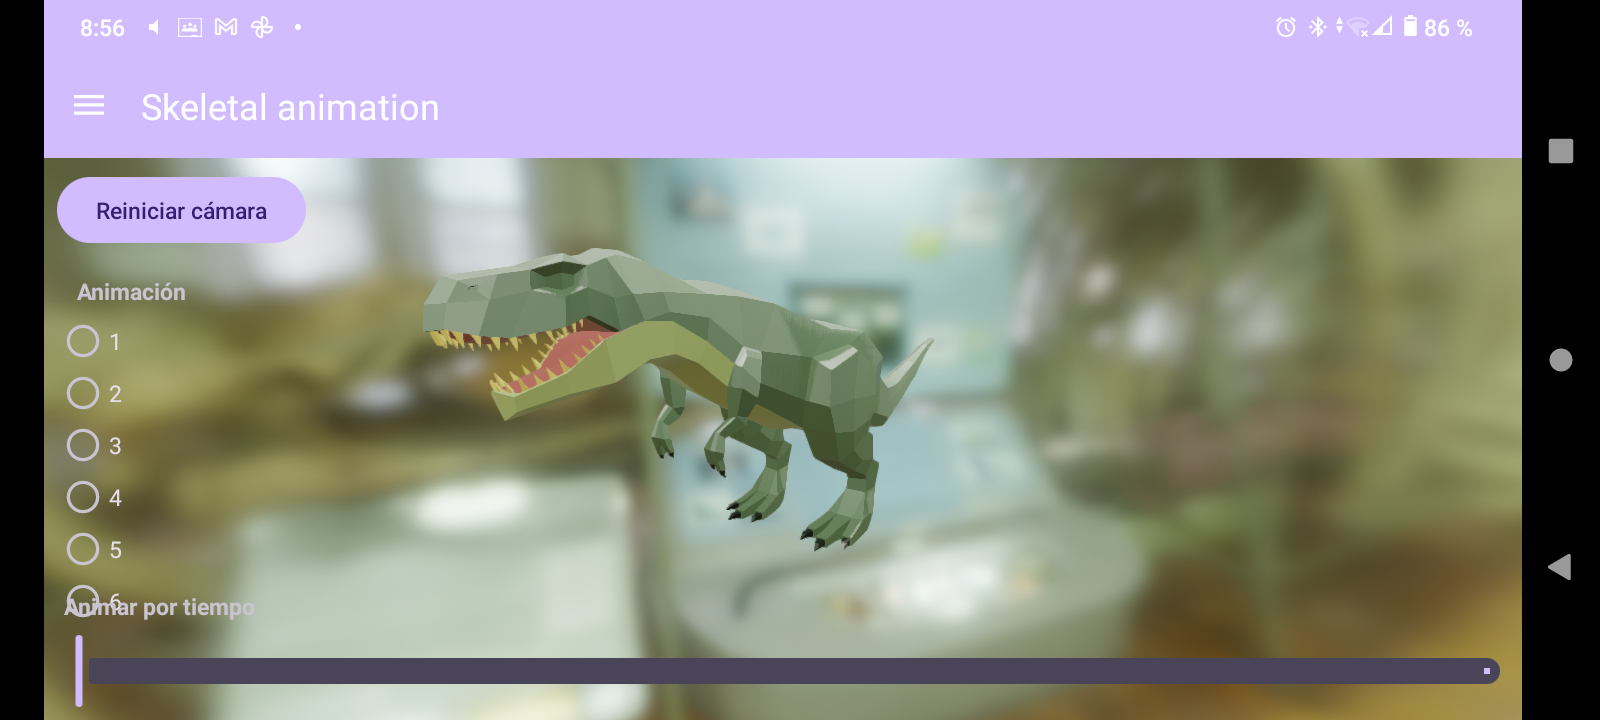
\includegraphics[width=0.45\textwidth]{img/Captura_5.png}
    \caption{Dinosaurio animado, mostrando otra instancia de animación esquelética.}
    \label{fig:modelo_dinosaurio}
\end{figure}

\subsection{Optimización del Rendimiento}

Las pruebas realizadas en dispositivos de gama media y baja confirmaron que la aplicación mantiene un rendimiento estable, sin caídas significativas de cuadros por segundo. Las optimizaciones implementadas, como la reducción de polígonos y la compresión de texturas, permitieron que los modelos se cargaran rápidamente y sin problemas visuales.

\begin{figure}[H]
    \centering
    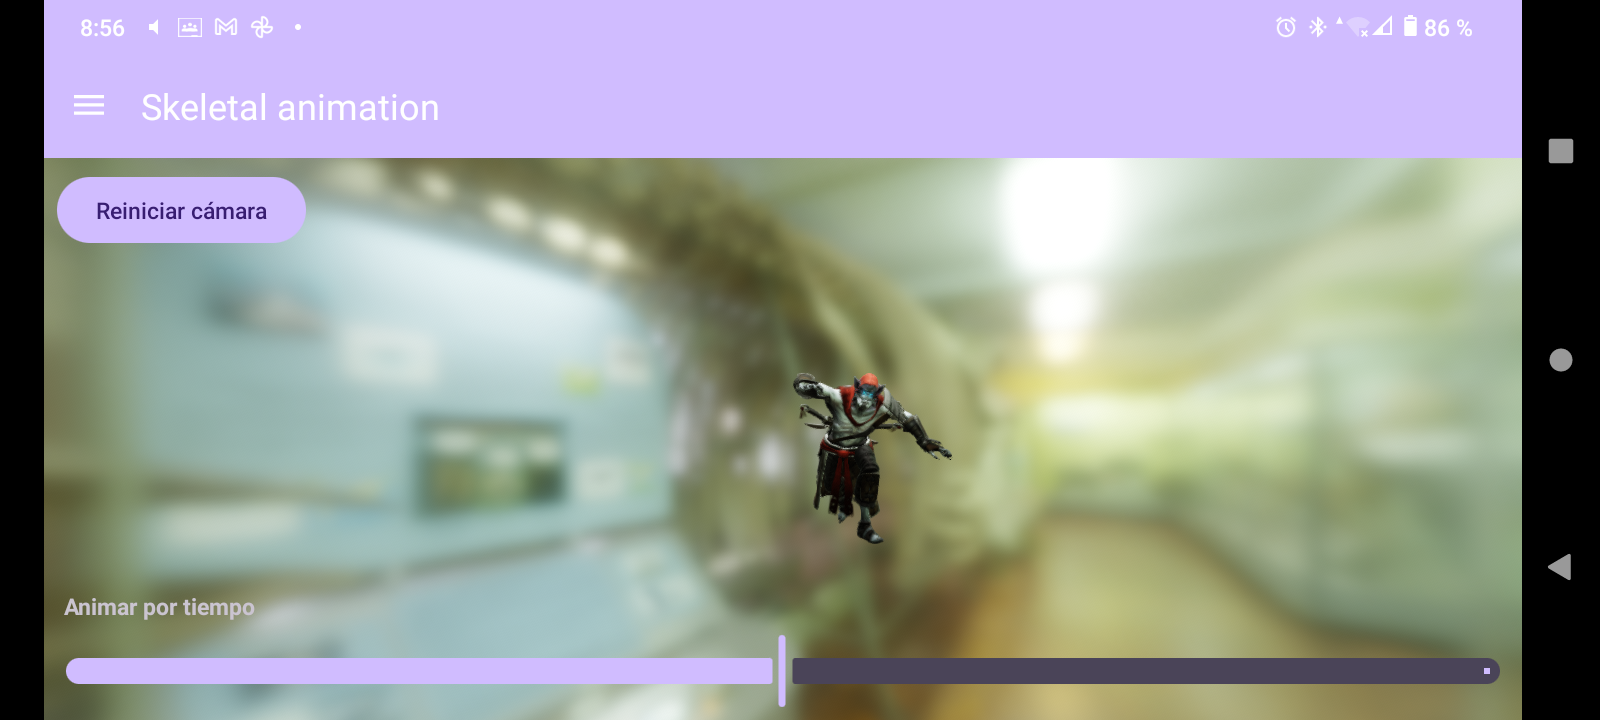
\includegraphics[width=0.45\textwidth]{img/Captura_4.png}
    \caption{Modelo en ejecución en un entorno optimizado para dispositivos móviles.}
    \label{fig:rendimiento}
\end{figure}

\subsection{Interacción con los Modelos 3D}

Los usuarios pueden rotar, hacer zoom y mover la cámara alrededor de los modelos, lo que facilita la exploración desde diferentes ángulos. Esta funcionalidad se logró mediante la implementación de gestos táctiles intuitivos, los cuales respondieron bien durante las pruebas.

\begin{figure}[H]
    \centering
    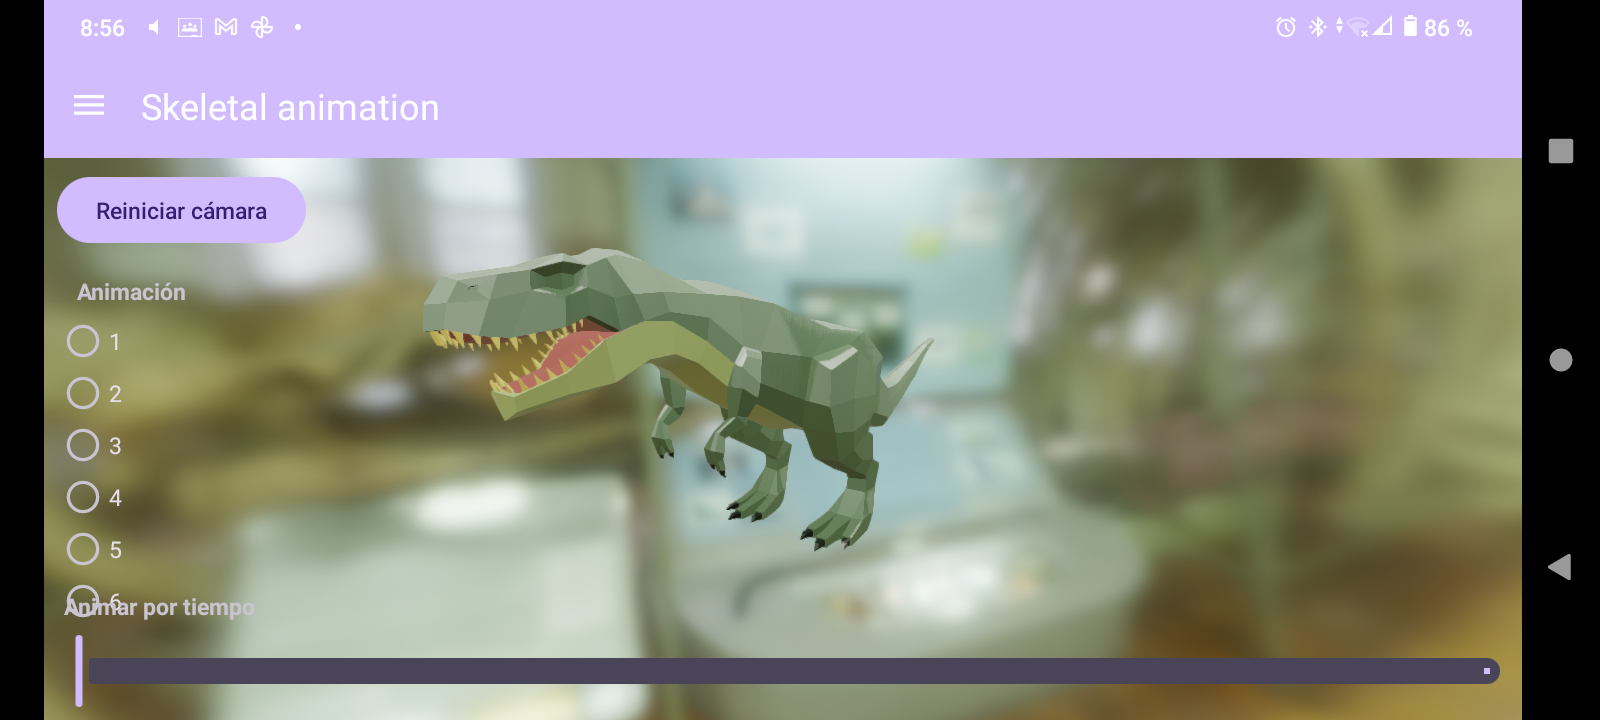
\includegraphics[width=0.45\textwidth]{img/Captura_5.png}
    \caption{Control de cámara mediante gestos táctiles.}
    \label{fig:gestos_tactiles}
\end{figure}

\subsection{Pruebas de Animaciones}

Las animaciones fueron probadas en diversos tiempos utilizando el control deslizante. Las pruebas demostraron que las transiciones entre diferentes tiempos y animaciones eran fluidas y sin interrupciones.

\begin{figure}[H]
    \centering
    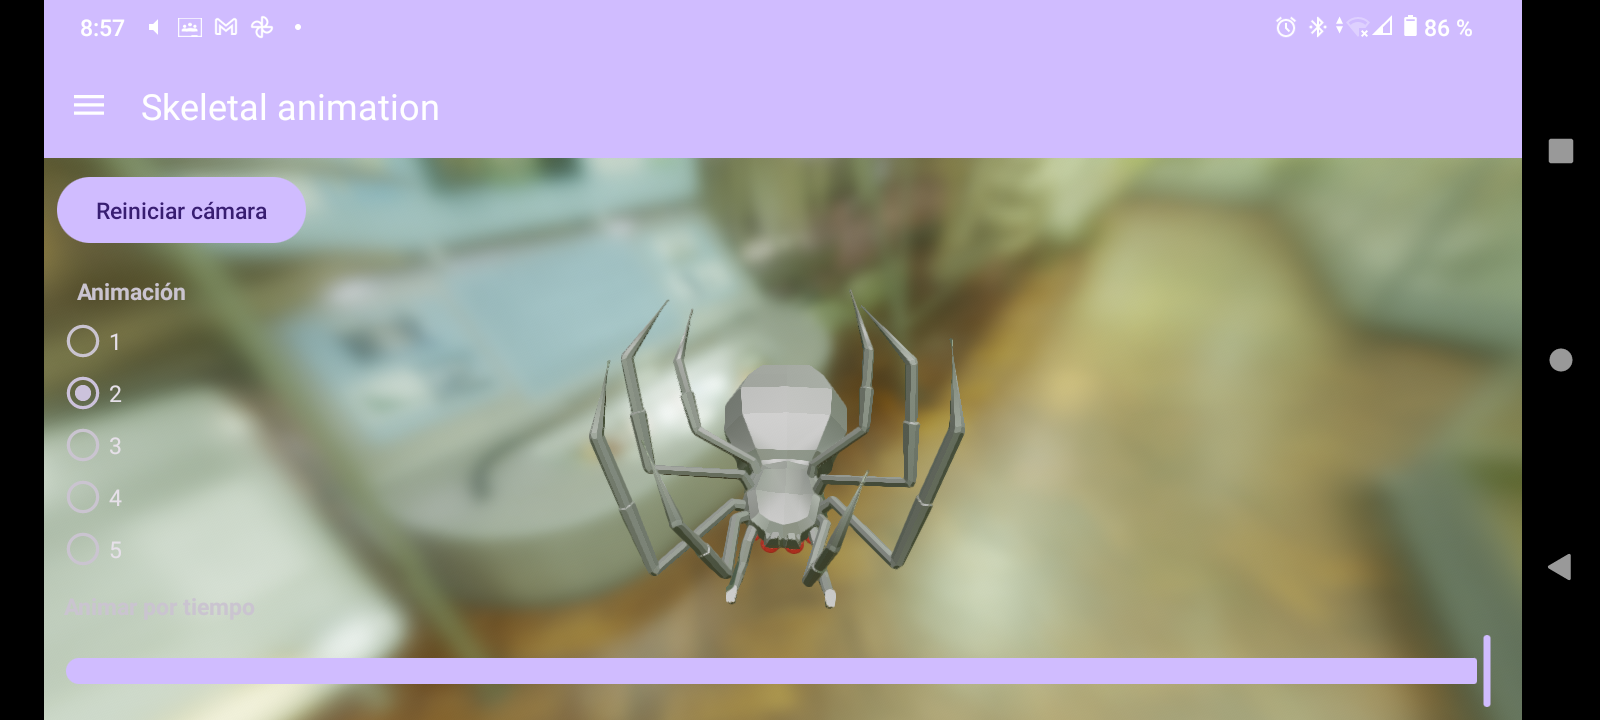
\includegraphics[width=0.45\textwidth]{img/Captura_13.png}
    \caption{Cambio de animación utilizando el control deslizante.}
    \label{fig:control_animacion}
\end{figure}

\subsection{Conclusión Visual}

Los shaders aplicados mejoraron la calidad visual de los modelos, añadiendo sombras y efectos de iluminación que proporcionaron un mayor realismo a la escena. Los modelos, incluso en movimiento, conservaron su integridad visual y los detalles en texturas y animaciones.

\begin{figure}[H]
    \centering
    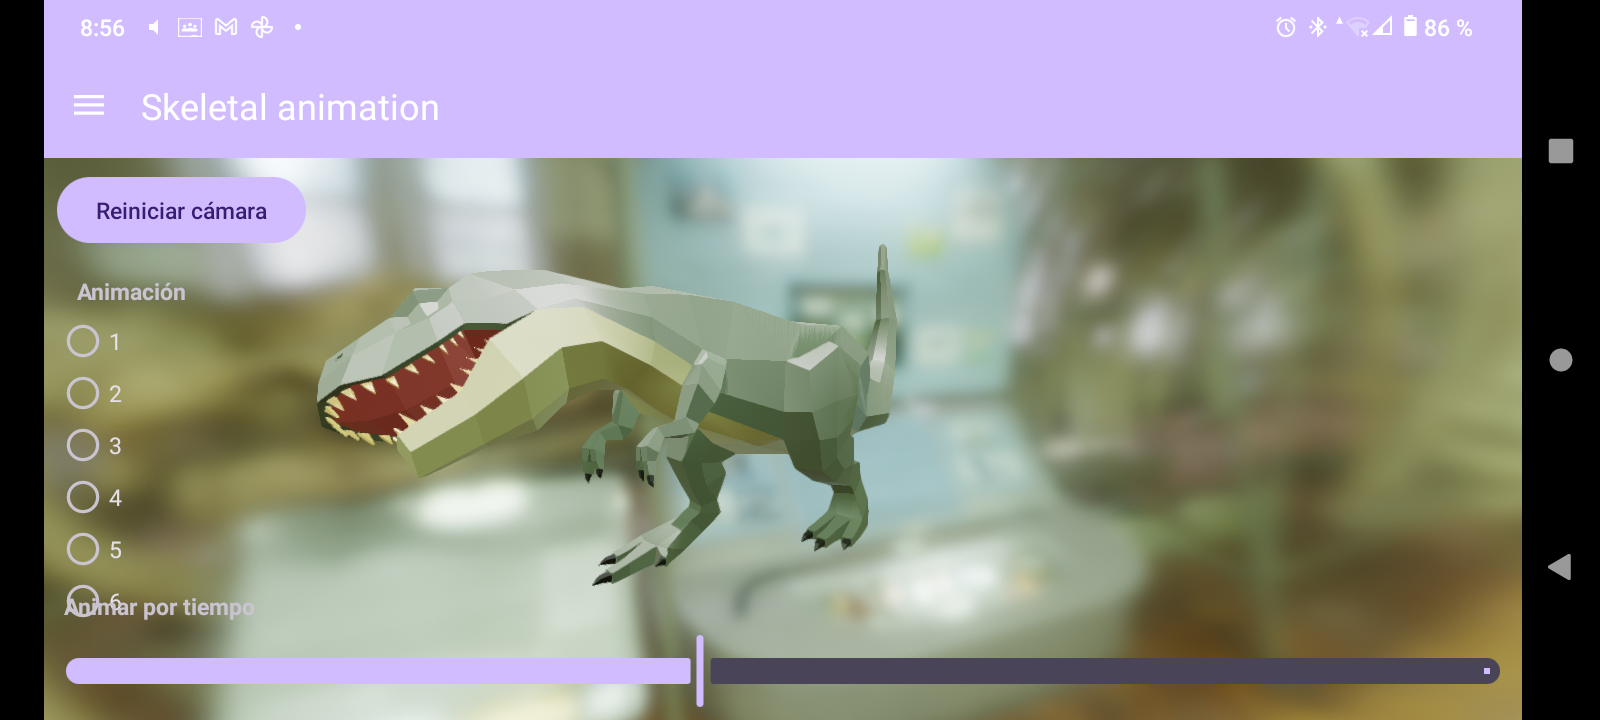
\includegraphics[width=0.45\textwidth]{img/Captura_7.png}
    \caption{Detalle visual mejorado gracias a la implementación de shaders.}
    \label{fig:detalle_visual}
\end{figure}

\begin{figure}[H]
    \centering
    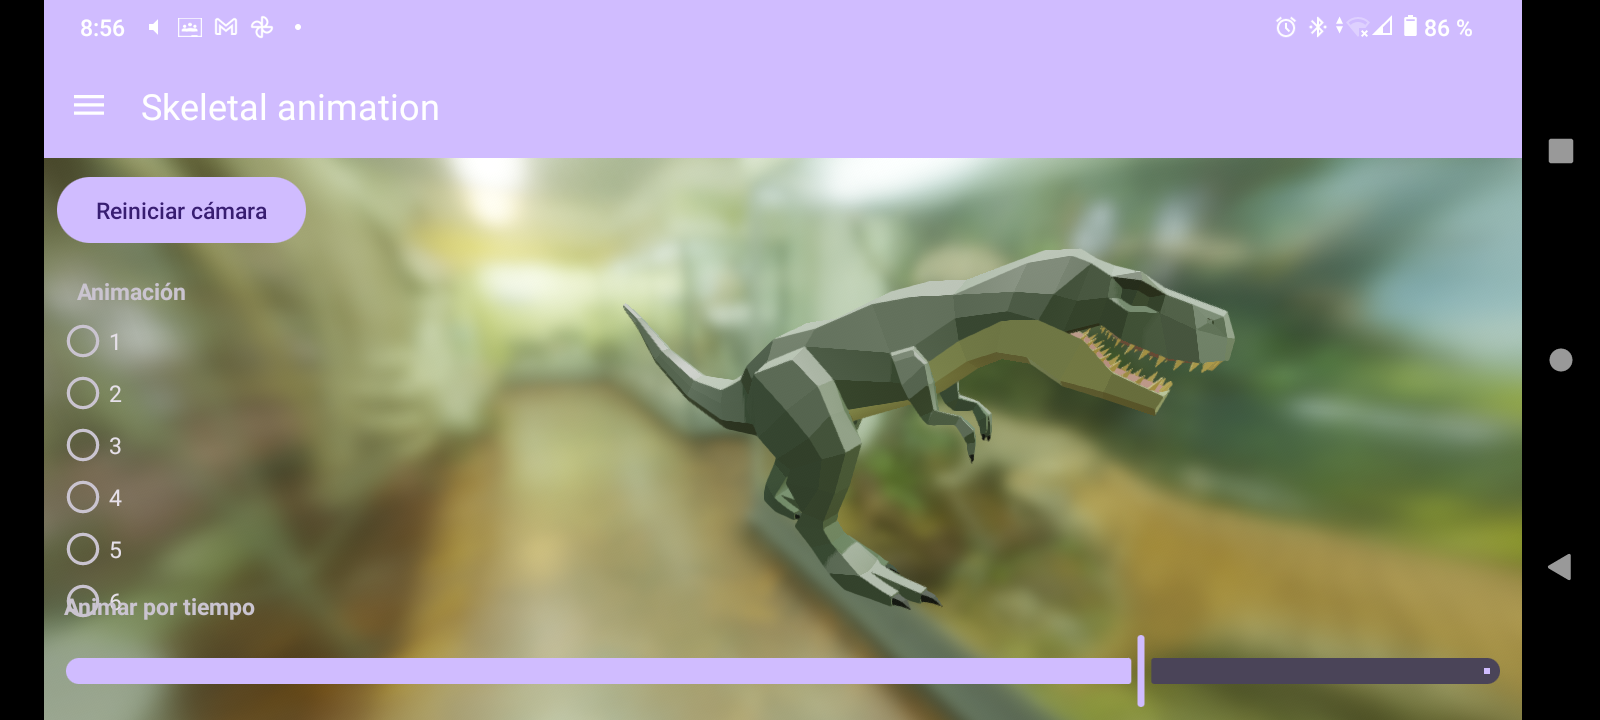
\includegraphics[width=0.45\textwidth]{img/Captura_8.png}
    \caption{Vista final del modelo con efectos de iluminación avanzados.}
    \label{fig:iluminacion_avanzada}
\end{figure}

Las imágenes incluidas ilustran las funcionalidades descritas y evidencian el éxito del proyecto en términos de implementación técnica y usabilidad. La aplicación cumple con el objetivo de ser una herramienta para visualizar y manipular modelos 3D animados en tiempo real, con potencial para futuras expansiones.

%%%%%%%%%%%%%%%%%%%%%%%%%%%%%%%%%%%%%%%%%%%%%%%%%%%%
\section{Conclusión}  

El desarrollo de esta aplicación móvil para la visualización y animación de modelos 3D utilizando el motor de renderizado Filament y OpenGL demostró ser un proyecto exitoso, logrando cumplir con los objetivos planteados. Se destacan los puntos más relevantes: \cite{mobileRendering}

\begin{itemize}
    \item Se logró crear una aplicación funcional e intuitiva que permite a los usuarios visualizar modelos 3D con animaciones esqueléticas en tiempo real. La interfaz de usuario es sencilla y facilita la interacción mediante controles táctiles y opciones accesibles.
    \item La implementación de técnicas de optimización, como la reducción de polígonos y la compresión de texturas, permitió que la aplicación mantuviera un rendimiento estable incluso en dispositivos móviles de gama media y baja.
    \item Las animaciones esqueléticas se reprodujeron de manera precisa, sin distorsiones ni errores visuales, gracias al uso eficiente del motor Filament y la integración con OpenGL.
    \item Los efectos visuales avanzados, como la iluminación y las sombras generadas mediante shaders, añadieron un nivel de realismo y calidad gráfica destacable, mejorando la experiencia del usuario.
    \item Las pruebas realizadas validaron la funcionalidad de la aplicación, mostrando que las interacciones con los modelos 3D, la manipulación de la cámara y las transiciones entre animaciones eran fluidas y sin interrupciones.
\end{itemize}

En términos generales, este proyecto demostró cómo es posible aprovechar tecnologías modernas de renderizado para desarrollar aplicaciones gráficas avanzadas en dispositivos móviles. Sin embargo, aún hay espacio para mejoras futuras, como:

\begin{itemize}
    \item Integrar soporte para cargar modelos 3D dinámicamente desde fuentes externas, como internet.
    \item Añadir más opciones de personalización para las animaciones y los efectos visuales.
    \item Extender la compatibilidad con otros formatos de modelos 3D y motores de renderizado.
\end{itemize}

Este trabajo abre la puerta a nuevas aplicaciones interactivas en diversas áreas, como educación, entretenimiento y simulación, demostrando el potencial de las tecnologías móviles para soportar experiencias gráficas avanzadas y accesibles.


\addcontentsline{toc}{section}{Referencias} 
\printbibliography
\end{document}













